\documentclass[11pt,a4paper]{article}
\usepackage[margin=19mm,top=20mm,bottom=20mm]{geometry}
\usepackage{amsmath,amssymb,graphicx,array,fancyhdr,lastpage,textcomp,fancyvrb}
\usepackage{fontspec}
\usepackage[hidelinks]{hyperref}
\setmainfont{texgyreheros-regular.otf}[BoldFont=texgyreheros-bold.otf,ItalicFont=texgyreheros-italic.otf,BoldItalicFont=texgyreheros-bolditalic.otf]
\setmonofont{lmmono10-regular.otf}
\setlength{\parindent}{0pt}\setlength{\parskip}{5pt}
\setlength{\headheight}{14pt}
\pagestyle{fancy}\fancyhf{}
\renewcommand{\headrulewidth}{0.3pt}\renewcommand{\footrulewidth}{0.3pt}
\fancyfoot[L]{\footnotesize by paper.shrit.in\quad |\quad normal}
\fancyfoot[R]{\footnotesize Page \thepage\ of \pageref{LastPage}}
\begin{document}
\fancyhead[L]{\small Data Analytics}\fancyhead[R]{\small Set A: Ensemble}
{\LARGE\bfseries Worked Solutions}\par{\large Data Analytics}\par\textbf{Set A: Ensemble | CSE Semester 3}\par
Companion to \texttt{da-ensemble.pdf}. Question numbers match that paper. Equivalent correct methods are acceptable. These are independent worked solutions, not an official university marking scheme.\par\medskip\hrule\medskip
Questions 1--5: MCQ answer key, 1 mark each (5 marks total). Questions 6 onward: theory solutions (25 marks total).\par
\noindent\begin{minipage}{\linewidth}\subsection*{1. Null hypothesis}
\textbf{Correct option: (A).} The null hypothesis specifies the population parameter: $H_0:\mu=0.95$.
\end{minipage}\par\medskip
\noindent\begin{minipage}{\linewidth}\subsection*{2. Standard error}
\textbf{Correct option: (C).} $SE=\sigma/\sqrt n=0.02/\sqrt{36}=0.02/6$.
\end{minipage}\par\medskip
\noindent\begin{minipage}{\linewidth}\subsection*{3. Normal-test statistic}
\textbf{Correct option: (B).} $z=(0.947-0.95)/(0.02/6)=-0.90$.
\end{minipage}\par\medskip
\noindent\begin{minipage}{\linewidth}\subsection*{4. Equal-width bins}
\textbf{Correct option: (D).} Bin width is $(480-180)/3=100$.
\end{minipage}\par\medskip
\noindent\begin{minipage}{\linewidth}\subsection*{5. Equal-frequency bins}
\textbf{Correct option: (B).} Each bin contains $12/3=4$ observations.
\end{minipage}\par\medskip
\noindent\begin{minipage}{\linewidth}\subsection*{6. Descriptive statistics, preparation and ANOVA}

(i) $N=20$, $\sum x_i=1350$, $\bar x=67.5$, and the median is 63. Using the population denominator,
\[\sigma^2=\frac{\sum(x_i-67.5)^2}{20}=238.35,
\qquad \sigma=15.4386.\]
Pearson's second coefficient is $3(67.5-63)/15.4386=\boxed{0.8744}$, indicating positive skewness.

(ii) Combine quantity and unit price to create revenue: $\mathrm{revenue}=\mathrm{quantity}\times\mathrm{unit\ price}$. This gives a useful derived variable from two existing columns.

(iii) Test $H_0:\mu_A=\mu_B=\mu_C$ against at least one unequal mean. The group means are 3, 5 and 7; the grand mean is 5.
\[SS_B=4[(3-5)^2+(5-5)^2+(7-5)^2]=32,\quad SS_W=4+2+4=10.\]
\begin{center}\renewcommand{\arraystretch}{1.2}\begin{tabular}{lllll}\hline Source & SS & df & MS & F\\\hline
Between & 32 & 2 & 16 & 14.4\\
Within & 10 & 9 & 1.1111 & \\
Total & 42 & 11 &  & \\\hline\end{tabular}\end{center}Since $14.4>4.256$, reject $H_0$ at 5\%. Mean flavour ratings differ. The test alone does not identify which pairs differ.
\end{minipage}\par\medskip
\noindent\begin{minipage}{\linewidth}\subsection*{7. Box plot and Spearman correlation}

(i) Sorted observations:
\[42,47,50,50,54,58,60,61,62,63,63,68,75,78,78,79,82,91,92,97.\]
The five-number summary is $\boxed{(42,56,63,78.5,97)}$.
Here $Q_1=(54+58)/2=56$, $Q_3=(78+79)/2=78.5$, and $IQR=22.5$.
The fences are $22.25$ and $112.25$, so there are no outliers.
\begin{center}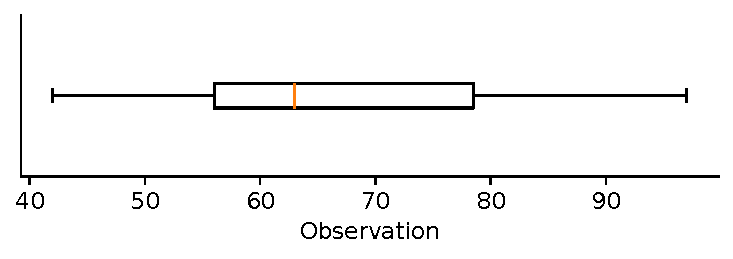
\includegraphics[width=.75\linewidth]{figures/box-source.pdf}\end{center}
(ii) Subsets support analysis of relevant cohorts, reduce computational load, and allow separate training and validation sets. Select them appropriately to avoid introducing bias.

(iii) The first two ranks agree. The other ten items have rank differences $\pm1$, so $\sum d_i^2=10$.
\[r_s=1-\frac{6(10)}{12(12^2-1)}=\boxed{0.9650}.\]
The interviewers have strong positive rank agreement.
\end{minipage}\par\medskip
\noindent\begin{minipage}{\linewidth}\subsection*{8. Left-tailed normal test}

Under the supplied model, $H_0:\mu=0.95$ and $H_1:\mu<0.95$.
\[z=\frac{0.93-0.95}{0.04/\sqrt{50}}=\boxed{-3.5355}.\]
Since $-3.5355<-1.645$, reject $H_0$. The evidence supports a mean accuracy below 95\% under this model ($p\approx0.000203$). The supplied standard deviation is treated as that of accuracy measurements, not inferred as a Bernoulli standard deviation from individual positive/negative results.
\end{minipage}\par\medskip
\noindent\begin{minipage}{\linewidth}\subsection*{9. Vaccination and disease: chi-square test}

$H_0$: vaccination status and disease status are independent. $H_1$: they are associated. Compute each expected count as row total times column total divided by 2000.
\begin{center}\renewcommand{\arraystretch}{1.2}\begin{tabular}{lll}\hline Group & Attacked: observed / expected & Not attacked: observed / expected\\\hline
Vaccinated & 31 / 54 & 469 / 446\\
Not vaccinated & 185 / 162 & 1315 / 1338\\\hline\end{tabular}\end{center}
\[\chi^2=\frac{23^2}{54}+\frac{23^2}{446}+\frac{23^2}{162}+\frac{23^2}{1338}
=\boxed{14.6432}.\]
There is one degree of freedom. Since $14.6432>3.841$, reject independence. The observed attack rates are $31/500=6.2\%$ and $185/1500=12.33\%$. Vaccination is associated with a lower attack rate in this sample; the table alone does not establish causation.
\end{minipage}\par\medskip
\noindent\begin{minipage}{\linewidth}\subsection*{10. Two-factor ANOVA with replication}

There are $a=3$ varieties, $b=4$ fertilizers and $r=2$ replicates per cell. The grand mean is $8.6667$. Variety means are $(8.5,7.25,10.25)$ and fertilizer means are $(8.1667,9.5,6.1667,10.8333)$.
Use
\begin{align*}
SS_A&=br\sum_i(\bar y_{i..}-\bar y)^2,\quad
SS_B=ar\sum_j(\bar y_{.j.}-\bar y)^2,\\
SS_{AB}&=r\sum_{i,j}(\bar y_{ij.}-\bar y_{i..}-\bar y_{.j.}+\bar y)^2,\\
SS_E&=\sum_{i,j,k}(y_{ijk}-\bar y_{ij.})^2.
\end{align*}
\begin{center}\renewcommand{\arraystretch}{1.2}\begin{tabular}{lllll}\hline Source & SS & df & MS & F\\\hline
Variety & 36.3333 & 2 & 18.1667 & 36.3333\\
Fertilizer & 71.3333 & 3 & 23.7778 & 47.5556\\
Interaction & 3.6667 & 6 & 0.6111 & 1.2222\\
Error & 6 & 12 & 0.5 & \\
Total & 117.3333 & 23 &  & \\\hline\end{tabular}\end{center}
Reject equal variety means because $36.3333>3.885$. Reject equal fertilizer means because $47.5556>3.490$. Both factors have significant effects at 5\% under the supplied assumptions. The interaction is retained in the model; its statistic is shown for completeness. The residual error mean square, rather than the interaction mean square, is the denominator for these fixed-factor tests.
\end{minipage}\par\medskip
\noindent\begin{minipage}{\linewidth}\subsection*{11. Cholesterol binning}

Range $=260-145=115$, so width $=115/3=38.3333$.
\begin{center}\renewcommand{\arraystretch}{1.2}\begin{tabular}{llll}\hline Method & Bin 1 & Bin 2 & Bin 3\\\hline
Equal width & [145,183.333): 7 & [183.333,221.667): 3 & [221.667,260]: 2\\
Equal frequency & 145,155,160,162 & 165,172,180,190 & 200,220,240,260\\\hline\end{tabular}\end{center}
For equal frequency, use boundaries 145, 163.5, 195 and 260. Equal width better displays the declining concentration across these data and the upper tail. Equal frequency gives balanced groups but requires density heights to make its unequal-width histogram meaningful.
\begin{center}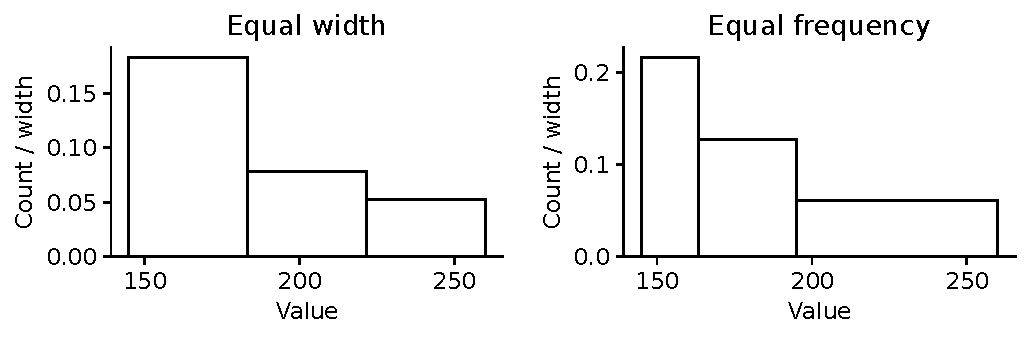
\includegraphics[width=.85\linewidth]{figures/bins-cholesterol.pdf}\end{center}
\end{minipage}\par\medskip

\end{document}
